\section{Background}

\subsection{Objective}

The interest in conducting this thesis research started with a series of
articles published by researchers at Google in their research blog
\cite{gu2016deep,finn2016deep,yahya2016collective,chebotar2016path}. The main
theme in these articles was robotic manipulation learned by gathering
experience in real time in non-simulated contexts. In two of these articles
\cite{gu2016deep,finn2016deep} tasks are learned from scratch without the need
for initializing by demonstration. Although, in the article by Gu et al.
\cite{gu2016deep}, poses of targets and arms are known from attached equipment.
It would be interesting to incorporate estimation of poses from visual feedback
in this case to lessen the need for external equipment. Another central theme
in these articles is the distributed collection of experience over several
robots. This is done in order to decrease the time it takes to collect data and
to increase variance of the data and the robustness of the algorithms. The use
cases for incorporating and extending these findings could be robotic
manipulation tasks with camera as feedback where exact relative positions of
objects, manipulators, and sensors need not be fixed. Also, where resources
exists to use several robots for speeding up the learning process. Possible
readers might be other researchers working with end-to-end machine learning for
robotic manipulation. Other interested parties might also be manufacturers
where repetitive tasks are a part of the production chain and variations in
these make it hard for robots to be easily programmed for those tasks.

\subsection{Reinforcement learning}

This entire section is descriptions of key concepts from a book on
Reinforcement Learning by Sutton and Barto \cite{sutton1998reinforcement}.

\subsubsection{The three tiers of machine learning}

In reinforcement learning (RL) an agent interacts with an environment and tries
to maximize how much \textit{reward} it can observe from the environment. To
maximize the reward in the long run might require short-time losses, making the
problem more complex than just maximizing for one step at a time. To find a
good strategy, commonly referred to as a \textit{policy}, the agent uses its
experience to make better decisions, this is referred to as
\textit{exploitation}. But, it must also find a balance between exploitation
and to also try out new things, i. e. \textit{exploration}. These things are
specific for RL and therefore distinguishes it from supervised and unsupervised
learning making it the third piece of machine learning.

\subsubsection{Main elements of RL}

Let $S_t$ be the state at time $t$, $R_t$ be the reward at time $t$, and $A_t$
the action at time $t$. The interaction between an agent and its environment in
RL is depicted in figure \ref{fig:rl_flowchart}. At time step $t$, the agent reads
the environment state and takes an action. The environment changes, maybe
stochastically, by responding with a new state and a reward at time $t+1$. 

\begin{figure}[h]
    \centering
    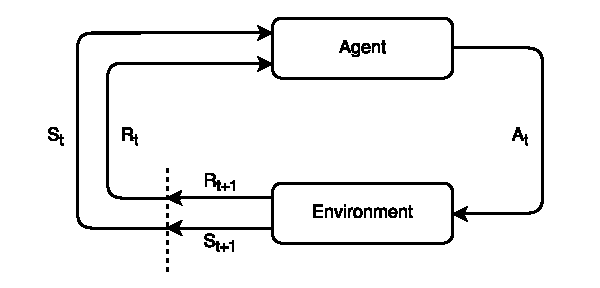
\includegraphics[]{res/agent_environment_interaction.pdf}

    \caption{Agent and environment interaction in RL. $S_t$, $R_t$, and $A_t$
             is the state, reward, and action at time $t$.}

    \label{fig:rl_flowchart}
\end{figure}

The quantity to maximize is often not the individual rewards, but rather the
long term accumulated rewards. Let us call this quantity $G_t$, or
\textit{return}, for an agent at time $t$:

\begin{equation}
    G_t = \sum_{k=0}^\infty \gamma^k R_{t+k+1}
\end{equation}

Some problems imply infinite sequences of actions and rewards and in turn
implying that the sum of all rewards be infinite. It is of course a problem to
maximize something infinite and that is the reason for the $\gamma \in \left[0, 1\right]$ factor above
that alleviates this problem if $\gamma < 1$. For lower values of $\gamma$ the agent
tries to maximize short term rewards, and for larger values long-term rewards. 

A policy is a function from the state of the environment to probabilities over
actions, i. e.  the function that chooses what to do in any situation. Since a
reward is only short-term, a \textit{value function} tries to estimate the
total amount of reward that will be given in the long run for being in some
state and following some policy. To enable planning of actions in the
environment, RL algorithms sometimes uses a \textit{model} in order to try out
actions in this before making decisions. This is usually referred to as
\textit{model-based} RL in contrast to \textit{model-free}. TODO: Change "try
out" above if not correct.

\subsubsection{Finite Markov Decision Processes}

In a RL scenario where the environment has a finite number of states, there is
a finite number of actions, and the Markov property holds is called a
\textit{finite Markov Decision Process} (finite MDP). The dynamics of a finite MDP is completely specified by the
probability distribution:

\begin{equation}
    p(s', r|s, a) = P(S_{t+1} = s', R_{t+1} = r | S_t = s, A_t = a)
\end{equation}

Important functions and terminology that is used throughout RL includes the \textit{state-value function} (abbreviated as value function) and
the \textit{action-value function}. The state-value function with respect to some policy informally tells you
how good a state is to be in given that you follow that policy:

\begin{equation}
    v_\pi(s) = \mathbb{E}_\pi\left[G_t|S_t=s\right] = \mathbb{E}_\pi\left[\sum_{k=0}^\infty \gamma^k R_{t+k+1}|S_t=s\right]
\end{equation}

To compare the value of different actions in some state, given that you thereafter follow some policy $\pi$,
is given by the action-value function:

\begin{equation}
    q_\pi(s, a) = \mathbb{E}_\pi\left[G_t|S_t=s,A_t=a\right] = \mathbb{E}_\pi\left[\sum_{k=0}^\infty \gamma^k R_{t+k+1}|S_t=s,A_t=a\right]
\end{equation}

According to RL theory there is always an optimal policy, i. e. that gives the
highest possible expected return given any state. This is often denoted with
$*$ and has the corresponding value and action-value functions $v_*(s)$ and
$q_*(s, a)$. Given the optimal value or action-value function, it is (depending
on the problem) easy to infer the optimal policy, therefore a common approach
is to first approximate either of these functions.

\subsubsection{Policy and value iteration}

One exact method to find the optimal policy, at least in the limit, is called
\textit{policy iteration}. This builds on two alternating steps, the first
called \textit{iterative policy evaluation}. This estimates a value function
given some policy and starts from a random value function $v_0$, except for any
terminal state which is assigned $0$. Then we iteratively update new value
functions for each step:

\begin{align*}
    v_{k+1}(s) &= \mathbb{E}\left[R_{t+1} + \gamma v_{k}(S_{t+1}) | S_t=s \right] \\
               &= \sum_a \pi (a|s) \sum p(s', r|s, a) \left[r + \gamma v_k(s')\right]
\end{align*}

As can be seen, the dynamics $p(s', r|s, a)$ needs to be known, which of course
is not always the case. The next step is called \textit{policy improvement} and for this
we first need to calculate the action-state function given the current policy
$\pi$:

\begin{align*}
    q_\pi(s, a) &= \mathbb{E}\left[R_{t+1} + \gamma v_\pi(S_{t+1}) | S_t=s, A_t = a \right] \\
                &= \sum_{s', r} p(s', r|s, a) \left[r + \gamma v_\pi(s')\right]
\end{align*}

When we have this, we can get an improved policy $\pi'$ by:

\begin{equation}
    \pi'(s) = \text{arg}\max_a q_\pi(s, a)
\end{equation}

Iteratively doing these two steps will eventually converge to the optimal
policy. There is an alternative way that is done by only approximating the
value function, called \textit{value iteration}:

\begin{align*}
    v_{k+1}(s) &= \max_a \mathbb{E}\left[R_{t+1} + \gamma v_k(S_{t+1}) | S_t=s, A_t = a \right] \\
             &= \max_a \sum_{s', r} p(s', r|s, a) \left[r + \gamma v_k(s')\right]
\end{align*}

\subsubsection{Monte Carlo methods and Time Difference learning}

Policy and value iteration are exploring the entire state-action space and
finds an optimal policy if the dynamics of the environment are known. Sometimes
we are dealing with samples from interacting with a system, and where we do not
know the dynamics. For these cases, we can instead estimate the action-value
function given a policy. This can be done by \textit{Monte Carlo methods} which
basically is averaging of returns for samples that we have attained. The other
method is \textit{Time difference methods} which estimates an error for each
observed reward and updates the action-value function with this. To be more
precise, one famous example of a time difference method is \textit{Q-learning}
and the updates are done according to:

\begin{equation}
    Q(S_t, A_t) \leftarrow Q(S_t, A_t) + \alpha \left[ R_{t+1} + \gamma \max_a Q(S_{t+1}, a) - Q(S_t, A_t) \right]
\end{equation}

Q-learning is an example of an \textit{off-policy} method. This means that you
can use a second, or derived, policy for exploration, but the algorithm still
finds the greedy optimal policy. The other family of methods is called
\textit{on-policy} methods. In this case, the exploring policy is the
same as the policy being improved.

\begin{figure}
    \centering
    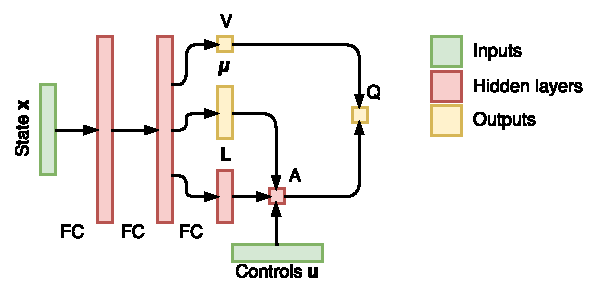
\includegraphics[width=0.6\textwidth]{res/naf-net.pdf}
\end{figure}

\subsection{Pilot study}

The following sections are the preliminary sources of information that was the
initial spark for this thesis as mentioned above. How to re-implement these
articles is not self-contained, so the pilot would necessarily need to also
include reading into articles from the references of these. Reading of these
initial articles would be needed to motivate an appropriate method, and then
further research would be done with the purpose of gaining all the information
needed to implement such a solution. The thesis study will be conducted at the
Robotics, Perception, and Learning lab at KTH with the main interest originally
being to dig into these articles and develop something further.

\subsubsection{Motion planning by ''Deep visual foresight''}

This article \cite{finn2016deep} trains a convolutional neural network on
images together with motion as inputs to predict how the image will change due
to that motion. This is later used to plan movement of objects to some target
pose.

\subsubsection{Path Integral Guided Policy Search}

In this article \cite{chebotar2016path}, the authors extend Guided Policy
Search and demonstrate two manipulation tasks. These are initialized from
demonstrations. To be able to comprehend this article, referenced articles
\cite{levine2016end,theodorou2010generalized,montgomery2016guided} would have
to be read as well.

\subsubsection{Collective Robot Reinforcement Learning with Distributed
               Asynchronous Guided Policy Search}

This article \cite{yahya2016collective} distributes learning of
door opening across several robots. The exact nature of the tasks
are varied across robots to increase robustness. The learning is
initialized from demonstration.

\subsubsection{Parallelized training without prior demonstration}

This article \cite{gu2016deep} shows several robotic manipulation tasks where
learning is parallelized across platforms, and they do not require previous
demonstrations.  For this article, I would need to read up on an algorithm
called Normalized Advantage Function (NAF) \cite{gu2016continuous}. In both of
the two previously mentioned articles
\cite{chebotar2016path,yahya2016collective} pose estimation of targets and
robots are done through visual feedback, while in this article
\cite{gu2016deep} no sensory feedback is provided and poses are known through
attached equipment. The pose estimation was done using a convolutional neural
network which could be a feasible extension to this article.


\subsubsection{Reinforcement learning}

These articles mentioned above naturally deals with reinforcement vocabulary
and assumes knowledge in this area. Therefore the pilot would include studying
a book by Sutton and Barto \cite{sutton1998reinforcement}. In this book,
chapters 1-3 and a section about non-linear function approximators are
essential (by advice from supervisor).

\subsection{Problem statement}

Manipulation tasks that seem trivial to a human can be hard to learn for
robots, especially from scratch without initial human demonstration due to high
sample complexity. Recent research suggests ways to do this but are based on
that you know the poses of the objects and the end-effector. For some scenarios
these are non-trivial to find out.

Problems also arise when learning in real time by collecting experience. Robots
must be able to evaluate their policies regularly at a high rate which is
complicated by adding a deep convolutional neural network for pose detection.
Also, learning tasks within a feasible time frame is harder when data
collection and policy updates happen in real time. The approach of
distributing collection of experience over several robots will be evaluated in
this thesis for handling this problem.

\subsection{Research question}

How can deep and distributed reinforcement learning be used for learning and
performing dynamic manipulation tasks with unknown poses.

\subsection{Expected scientific results}

If all goes well, previous results are verified in new contexts. Also
they are extended to also handle unknown target and manipulator poses.
